\documentclass[11pt,a4paper]{article}

\usepackage{amsmath}
\usepackage{amsfonts}
\usepackage{geometry}
\usepackage{graphicx}
\usepackage{fancyhdr}
\usepackage{setspace}
\usepackage{amssymb}
\usepackage{booktabs}
\usepackage{enumitem}
\usepackage{multirow}
\usepackage{titlesec}
\usepackage{caption}
\usepackage{subcaption}
\usepackage{float}

\setcounter{secnumdepth}{4}

% set table of content depth
\setcounter{tocdepth}{3} 
\usepackage[titles]{tocloft}

% set spacing 
\setlength{\cftbeforesecskip}{10pt}

% Page layout settings
\geometry{
    a4paper,
    left=20mm,
    right=20mm,
    top=25mm,
    bottom=25mm
}

\usepackage{biblatex}
\addbibresource{Project_Report_References.bib}

%%%%%%%%%%%%%%%%%%%%%%%%%%%%%%%%%%%%%%%%%%%%%%%%%%%%%%%%%%%%%%%%%%%%%%
%%%%%%%%%%%%%%%%%%%%%%%%%%%%%%%%%%%%%%%%%%%%%%%%%%%%%%%%%%%%%%%%%%%%%%
\begin{document}
\singlespacing  % Set the document to single line spacing
\thispagestyle{empty} % Remove page number for the cover page

\begin{center}
{\bf \LARGE Approaches to Noise Resilient Quantum Circuit Design}\\[0.5cm]
    \textbf{Christian Wood} \\[0.2cm]
    \textbf{Student ID:} 710018541 \\[1cm]
\end{center}

\section*{Abstract}

\noindent 
One of the key challenges in quantum computing is designing quantum circuits, a task made difficult by their probabilistic behaviour and counter-intuitive nature. Various automated techniques have been proposed, with genetic algorithms emerging as a popular method. In the current NISQ era, noise poses a serious obstacle by introducing significant computational errors. By leveraging multi-objective evolutionary algorithms (MOEAs), our approach not only automates circuit design but also includes additional criteria to enhance performance under realistic noisy conditions. We present an a priori MOEA that adapts to the design of arbitrary circuits along with a novel circuit representation scheme. We demonstrate the method’s effectiveness by applying it to the 2 and 3-qubit Quantum Fourier Transform (QFT), showing that the evolved circuits perform better in noisy environments than the traditional QFT circuit.

\newpage
\thispagestyle{empty} 
\section*{Declaration}
I acknowledge the following uses of GenAI tools in this assessment: 

\begin{itemize}[label={\ $\square$\ }, leftmargin=*]
  \item I have used GenAI tools to:
  \begin{itemize}[label={\ $\square$\ }, leftmargin=*]
    \item develop ideas.
    \item assist with research or gathering information.
    \item help me understand key theories and concepts.
    \item identify trends and themes as part of my data analysis.
    \item suggest a plan or structure for my assessment.
    \item give me feedback on a draft.
    \item generate images, figures or diagrams.
    \item proofread and correct grammar or spelling errors.
    \item generate citations or references.
    \item Other: [please specify]
    \item[]
  \end{itemize}
  \item I have not used any GenAI tools in preparing this assessment.
\end{itemize}

\bigskip
I declare that I have referenced all use of GenAI outputs within my assessment in line with the University referencing guidelines.

\vspace{1em}
I certify that all material in this dissertation which is not my own has been identified. 

\vspace{5em}
{\bf\noindent Signature:} \hrulefill
\newpage

% Table of Contents
\tableofcontents 
\thispagestyle{empty} 
\newpage 

% Reset page numbering for main report
\clearpage
\pagenumbering{arabic} 

%%%%%%%%%%%%%%%%%%%%%%%%%%%%%%%%%%%%%%%%%%%%%%%%%%%%%%%%%%%%%%%%%%%%%%
%
%    Introduction (Background and Integrated Literature Review)
%
%%%%%%%%%%%%%%%%%%%%%%%%%%%%%%%%%%%%%%%%%%%%%%%%%%%%%%%%%%%%%%%%%%%%%%
\section{Introduction}
\subsection{Background on Quantum Computing and the NISQ Era}
Quantum computing represents a paradigm shift in computational capability, leveraging principles of quantum mechanics to perform calculations that are infeasible for classical computers. Unlike classical bits, which exist in binary states of 0 or 1, quantum bits (qubits) exploit superposition \cite{Gudder1970ASP}, allowing them to exist in a probabilistic combination of both states simultaneously. This property, alongside quantum entanglement \cite{horodecki2009quantum}, where qubits become interdependent regardless of physical distance, enables exponential parallelism in computation.\newline

The potential of quantum computing has been demonstrated through theoretical breakthroughs such as Shor’s algorithm \cite{Shor365700}, which exponentially accelerates integer factorisation, posing a significant threat to classical cryptographic systems. Similarly, Grover’s algorithm \cite{Khanal2021QuantumML} provides a quadratic speed-up for unstructured search problems. These algorithms showcase the transformative potential of quantum computing across domains such as cryptography, optimisation, and material simulation.\newline

Despite these advantages, practical quantum computing remains constrained by current hardware limitations. We are presently in what is known as the Noisy Intermediate-Scale Quantum (NISQ) era \cite{Preskill2018QuantumCI}, a term coined by John Preskill. This era is characterised by quantum processors with a relatively low number of qubits (hundreds to a few thousand) that suffer from high error rates and limited qubit connectivity. Unlike fault-tolerant quantum computers, which are expected to leverage quantum error correction to enable reliable computation, NISQ devices must operate under significant noise constraints, making algorithmic optimisation crucial.\newline

Two key challenges in NISQ computing are quantum noise 
 \cite{Clerk2008IntroductionTQ} and limited qubit connectivity \cite{Preskill2018QuantumCI}. Quantum noise results from environmental decoherence and gate errors, causing information loss over time. As circuit depth increases, accumulated noise degrades computation fidelity, making depth minimisation an essential goal for circuit design. Additionally, physical qubits are not universally connected, requiring SWAP gates to facilitate interactions between non-adjacent qubits. These SWAP gates introduce additional operations, further increasing circuit depth and reducing fidelity.\newline

Addressing these limitations requires both hardware advancements and software-driven optimisation techniques. One promising approach involves the use of Evolutionary Algorithms (EAs) \cite{Lukac2002EvolvingQC} to automate the design of quantum circuits that result in particular behaviours. This can further be extended through the use of Multi-Objective Evolutionary Algorithms (MOEAs) \cite{moein} to optimise quantum circuit design for a variety of goals by balancing competing objectives such as circuit depth, gate fidelity, and adherence to physical qubit constraints. By leveraging MOEAs, it becomes possible to evolve quantum circuits that are better suited for execution on NISQ-era hardware, improving computational accuracy while mitigating noise effects.\newline

This dissertation focuses on the application of MOEAs to optimise the Quantum Fourier Transform (QFT) circuit \cite{Jozsa1997QuantumAA}, a fundamental component in many quantum algorithms. Through an evolutionary approach, this work aims to generate optimised QFT implementations that reduce noise sensitivity and improve execution efficiency on contemporary quantum processors.\newpage

\subsection{Problem Statement}
The QFT is a cornerstone of quantum computing, underpinning a wide range of quantum algorithms, from Shor’s factorisation \cite{Shor365700} and quantum phase estimation \cite{O’Brien_2019} to algorithms in signal processing and quantum simulation. Its central role in these transformative applications highlights the necessity of efficient QFT implementations. However, the practical deployment of QFT circuits on real quantum hardware, particularly in the current NISQ era, faces significant challenges.\newline

Furthermore, features such as gate selection and parametrisation are critical for noise resilience. The choice of gates directly affects both the circuit’s depth and its error profile. However, designing quantum circuits by hand to balance these competing factors is extremely challenging, often leading to suboptimal designs that do not fully exploit the quantum advantage.\newline

Evolutionary Algorithms (EAs), and in particular Multi-Objective Evolutionary Algorithms (MOEAs), offer a promising solution to this design challenge. By simultaneously optimising multiple objectives, such as maximising fidelity, minimising circuit depth, and selecting noise-resilient gates, MOEAs provide a systematic approach to navigating the vast search space of circuit architectures. This automated method not only alleviates the complexity of manual circuit design but also uncovers non-intuitive configurations that better balance the competing accuracy and noise resilience requirements on NISQ hardware.

\subsection{Research Aims and Objectives}
The overall aim of this research is to develop an evolutionary framework for optimising QFT circuits for execution on Noisy Intermediate-Scale Quantum (NISQ) devices. In pursuing this aim, the research is organised around three principal objectives:

\subsubsection*{Objective 1 - Evolve Quantum Circuits that Replicate Target Behaviour:}
The first objective is to design an algorithm capable of evolving quantum circuits that replicate the behaviour of a given target circuit. In this work, the QFT is chosen as the focal point because of its central role in a wide variety of quantum algorithms, such as Shor’s algorithm and quantum phase estimation. The challenge is to construct a representation and a set of genetic operators that allow the evolutionary algorithm to generate candidate circuits whose output states closely approximate the ideal QFT transformation.

\subsubsection*{Objective 2 - Enhance Circuit Resilience through Multiple Optimisation Techniques:}
The second objective is to implement a variety of techniques aimed at producing circuit designs that are resilient to quantum noise. Specifically, we will explore three complementary approaches:
\begin{itemize}
    \item \textbf{Noise-Aware Evaluation:} Incorporating realistic noise models into the fitness evaluation to preferentially select circuits that perform robustly under hardware-specific noise conditions.
    \item \textbf{Circuit Depth Reduction:} Imposing a fitness penalty based on circuit depth to encourage the evolution of more compact circuits, thereby reducing the cumulative effect of noise and decoherence.
    \item \textbf{Combined Approach:} Integrating both noise-aware evaluation and depth reduction within a unified fitness function, seeking to balance the trade-offs between fidelity, resilience, and resource utilisation.
\end{itemize}

\subsubsection*{Objective 3 - Comparative Analysis Against Traditional QFT Circuits under Varied Noise Models:}
The third objective is to perform a systematic performance comparison between the evolved QFT circuits and conventional QFT implementations across a range of noise models. This analysis aims to assess:
\begin{itemize}
    \item Which optimisation approach (noise-aware, depth reduction, or the combined method) yields the highest noise resilience for specific noise profiles.
    \item The generalisability of the evolved circuits across different noise conditions, noting that circuits optimised for reduced depth might exhibit broader resilience, while those tuned with noise-aware evaluation could perform exceptionally under targeted noise scenarios.
\end{itemize}

In addition to these primary objectives, we will explore the behaviour of our approach across circuits of varying qubit counts to provide insights into its scalability. We also plan to investigate the potential to replicate other quantum circuit designs, though these efforts are considered supplementary to the core objectives.\newline

This multi-faceted approach is designed to systematically address the challenges imposed by quantum noise and hardware constraints, ultimately leading to practical, high-fidelity QFT circuits optimized for NISQ devices.

%%%%%%%%%%%%%%%%%%%%%%%%%%%%%%%%%%%%%%%%%%%%%%%%%%%%%%%%%%%%%%%%%%%%%%
%
%    Methodology & Implementation
%
%%%%%%%%%%%%%%%%%%%%%%%%%%%%%%%%%%%%%%%%%%%%%%%%%%%%%%%%%%%%%%%%%%%%%%
\section{Methodology \& Implementation}

This section describes the evolutionary algorithm framework used to design QFT circuits. It covers our encoding of candidate circuits, how circuit performance is quantified via fitness evaluation, the genetic operators used to evolve these circuits, and the criteria by which success is measured.

\subsection{Circuit Representation}
A central challenge in applying EAs to quantum circuit design is devising a representation that is both expressive and efficient. Our representation was developed with two principal goals in mind: (1) the ability to encode complex, parametrised, and non‐adjacent multi‐qubit gate operations, which are critical for tailoring circuits to specific noise models, and (2) the capacity to schedule gate operations concurrently, thereby reducing circuit depth to enhance noise resilience on NISQ devices.\newline

Our approach follows a layer‐based paradigm inspired by Lukac’s \cite{Lukac2002EvolvingQC} block-based representation. In our encoding, each candidate circuit (chromosome) is modelled as an ordered list of layers, where each layer corresponds to a discrete time step in the circuit’s execution. The length of each layer equals the number of qubits, ensuring that operations assigned to different qubits within the same layer are executed in parallel. This inherently minimises the overall circuit depth, a crucial parameter when mitigating the deleterious effects of noise.\newline

Within each layer, individual positions are occupied by gate specification strings. These strings serve as compact descriptors of quantum operations. For example, a single-qubit gate, such as the Hadamard is represented as “h(0)”, indicating its application on qubit 0, while parametrised gates include additional information, e.g., “rx(0,0.5)” specifies an X-rotation on qubit 0 with a rotation parameter of 0.5. In the case of multi-qubit gates (double-qubit or triple-qubit), the encoding extends to include partner indices. To prevent a qubit from being scheduled for more than one operation within the same time step, positions corresponding to qubits that serve as partners in a multi-qubit operation are marked with a control marker (“-”). In addition, a special “barrier” operation, denoted by “w”, is used to denote no-operation.\newline

The creation of a new layer is governed by the function create\_new\_layer, which randomly assigns a gate to each qubit slot based on a weighted probability distribution. Specifically, the “w” (barrier) gate is assigned a fixed weight of 0.25, while the remaining 0.75 probability is equally distributed among the available single-qubit, double-qubit, and triple-qubit gates. This probabilistic selection ensures that while idle operations occur with a reasonable frequency, the evolutionary process is still driven by a diverse set of non-trivial gate operations. When a double-qubit gate is selected, an additional free index is randomly chosen to serve as its partner, and the partner position is then blocked by placing a “-”. Similarly, triple-qubit gates select two partners (if available) to ensure that the gate acts on three distinct qubits. This automated assignment preserves the integrity of each layer and prevents overlapping operations on the same qubit.\newline

Once the chromosome is constructed as a list of layers, each gate specification string is parsed using a regular expression-based function (parse\_gate\_spec), which extracts the gate type and any parameters. The parsed information is then used to build a corresponding Qiskit QuantumCircuit object via a mapping table (build\_gate\_map). This table defines a lambda function for each gate type, which applies the correct Qiskit operation to the circuit. The conversion process implemented in the get\_circuits function iterates over each layer in the chromosome, applying the specified operations sequentially (i.e., layer by layer) while executing all operations within a layer concurrently.\newline

This representation is particularly amenable to genetic manipulation. Its modular, layer-based structure allows genetic operators to modify circuits at both the layer and gate levels as will be covered in Section 2.3.\newline

\begin{figure}[H]
    \centering
    \includegraphics[width=1\textwidth]{Project Report/Images/Chromosome.png}
    \caption{Quantum Circuit Chromosome}
\end{figure}

\begin{figure}[H]
    \centering
    \includegraphics[width=1\textwidth]{Project Report/Images/Circuit.png}
    \caption{Quantum Circuit}
\end{figure}

Figure 1 shows a representative chromosome, where each row corresponds to a layer and each entry within a row is a gate specification (e.g., “h(0)”, “cx(1,0)”, or “-” for blocked positions). Figure 2 presents the quantum circuit derived from this chromosome, demonstrating how sequential layers map onto discrete time steps and how parallel operations reduce overall circuit depth.\newline

In summary, our layer-based representation with its integration of mapping tables and explicit control markers provides a robust framework for encoding complex QFT circuits. It accommodates both parametrised operations and parallel execution, which are essential for designing circuits that are both accurate and resilient to noise on current quantum hardware.

\subsection{Fitness Evaluation}
A fundamental aspect of any evolutionary algorithm (EA) is the fitness function, which defines the selection pressure guiding the evolutionary process. The design of this function plays a crucial role in shaping the fitness landscape and, consequently, the convergence behaviour of the algorithm. In this research, the fitness function must effectively evaluate evolved quantum circuits based on three key objectives:

\begin{enumerate}
    \item Accurately replicating the behaviour of the QFT.
    \item Assessing circuit performance under realistic noise conditions.
    \item Exploring strategies to enhance noise resilience by optimising circuit structure.
\end{enumerate}

To achieve these goals, multiple fitness evaluation strategies were explored, after which we decided to settle on Qiskit's state\_fidelity.

\subsubsection*{Fitness Evaluation Using State\_fidelity:}
A key component of our fitness evaluation relies on the \texttt{state\_fidelity} \cite{state_fidelity} function provided by Qiskit. This function computes how closely two quantum states align with each other. Mathematically, when the inputs are density matrices $\rho_1$ and $\rho_2$, fidelity is defined by

\[
\mathcal{F}(\rho_1, \rho_2) \;=\; 
\mathrm{Tr}\!\Bigl[\sqrt{\rho_1^{1/2}\,\rho_2\,\rho_1^{1/2}}\,\Bigr]^2
\]

In our study, we use this function to compare the output state of the evolved circuit against the ideal QFT-transformed state. Specifically, we apply the circuit to each of the $N = 2^{(\text{number of qubits})}$ computational basis states, compute the fidelity for each, and then average these values to obtain an overall measure of performance:

\[
F_{Base} \;=\;
\frac{1}{N}\sum_{i=1}^{N} \,
\mathcal{F}\bigl(\,\rho_{\mathrm{ideal}}^{(i)}, \,\rho_{\mathrm{circuit}}^{(i)}\bigr)
\]

This averaging ensures that our fitness metric captures the circuit's behaviour across the entire state space rather than focusing on a single initial state or a narrow subset.\newline

By using \texttt{state\_fidelity} in this manner, we obtain a robust, phase-sensitive metric that drives the evolutionary algorithm to discover QFT implementations capable of preserving fidelity under both ideal and noisy conditions.

Initially, no noise models were included in the fitness evaluation, allowing us to focus purely on evolving circuits that optimally implement the QFT transformation without external perturbations, thereby establishing a baseline for further experimentation.\newline

An alternative approach could have been to use a fitness function that solely captures phase, as this would be the most direct way to optimise QFT-specific behaviour. However, we opted against this for two primary reasons. First, \texttt{state\_fidelity} already fully captures phase accuracy while also accounting for amplitude, making an additional phase-specific metric redundant. Secondly, using \texttt{state\_fidelity} enhances the generalisability of our approach, allowing us to apply the same fitness function to assess performance on any other quantum circuit without modification. This flexibility is crucial for exploring broader applications beyond QFT.

\subsubsection*{Expanding the Fitness Function to Incorporate Circuit Depth and Noise:}
While optimising for noiseless \texttt{state\_fidelity} is effective for idealised conditions, quantum circuits deployed on NISQ experience significant degradation due to environmental decoherence and gate errors. To evaluate and enhance noise resilience, we incorporated additional fitness function variants, each designed to address a specific research question.

\paragraph*{Fidelity Optimisation with Circuit Depth Considerations:\newline}
Another approach to mitigating noise is to minimise circuit depth, as deeper circuits accumulate more errors due to prolonged coherence times and increased gate noise. To incorporate this, we introduced a depth penalty term:

\begin{equation}
    F_{DepthReduced} = F_{Base} - \lambda D
\end{equation}

where $D$ is the circuit depth and $\lambda$ is a penalty coefficient that controls the trade-off between fidelity and depth.

By reducing depth, this variant encourages solutions that are more efficient and less susceptible to noise accumulation, even if no explicit noise model is applied.

\paragraph*{Fidelity Optimisation with Noise Simulation:\newline}
To measure the impact of real-world quantum noise, we incorporated hardware-specific noise models into the fitness evaluation. Using Qiskit's AerSimulator with noise data extracted from IBM Quantum backends, we computed \texttt{state\_fidelity} under noisy conditions. This modified fitness function is given by:

\begin{equation}
    F_{Noisy} =  \;=\;
\frac{1}{N}\sum_{i=1}^{N} \,
\mathcal{F}\bigl(\,\rho_{\mathrm{ideal}}^{(i)}, \,\rho_{\mathrm{noisy}}^{(i)}\bigr)
\end{equation}

where $|\phi_{noisy}\rangle$ is the evolved circuit’s output when executed on a noisy simulator. This variant allows us to identify circuits that maintain high fidelity despite noise, prioritising solutions that are naturally robust to quantum errors.\newline

As part of the noise-simulated fitness, we incorporated a custom noise model that rigorously emulates the error mechanisms encountered in contemporary quantum hardware. This model integrates both depolarizing and damping error channels to capture a realistic noise environment. Specifically, depolarizing errors are applied to all gates, with each gate type assigned an error rate derived from empirical values observed in current quantum systems. In addition, amplitude damping and phase damping channels are included to simulate the relaxation and dephasing processes, respectively. These damping errors contribute to a cumulative degradation of state fidelity, an effect further exacerbated by increased circuit depth. Thus, the overall impact of noise is intrinsically linked to the circuit's architecture, emphasising the necessity for design strategies that mitigate error accumulation.


\paragraph*{Combined Fidelity, Noise, and Depth Optimisation:\newline}
The final variant integrates both noise simulation and depth penalties into the fitness function:

\begin{equation}
    \mathcal{F}_{NoisyDepthReduced} = F_{Noisy} - \lambda D
    \label{eq:1}
\end{equation}

This function simultaneously rewards high fidelity, noise resilience, and low circuit depth, producing solutions that are optimised for execution on real hardware.

\subsection{Genetic Operators}
The evolutionary process employed in this work leverages a set of genetic operators that produce a new generation of candidate solutions. These operators are central to effectively exploring the solution space and are composed of three key steps: parent selection, crossover, and mutation. In what follows, we describe each operator in detail and explain how they are integrated with our layered circuit representation.

\subsubsection*{Parent Selection:}
Parent selection is the first step in generating offspring, and its effectiveness is critical for maintaining both convergence speed and population diversity. In our experiments, we investigated several selection strategies, including:
\begin{itemize}
    \item \textbf{Random Parent Selection:} Candidates are chosen uniformly at random from the population, without any bias toward higher fitness.
    \item \textbf{Fitness Proportionate Selection:} Each candidate’s selection probability is proportional to its fitness value.
    \item \textbf{Fitness Proportionate Elitist Selection:} A variant that guarantees the best-performing individuals are retained.
    \item \textbf{Tournament Selection:} A subset of candidates is randomly sampled and the best among them is chosen.
    \item \textbf{Tournament Selection Elitist:} A version that always preserves the top performers from each tournament.
    \item \textbf{Rank Selection:} Candidates are ranked based on fitness, and selection probabilities are assigned linearly according to their rank.
    \item \textbf{Rank Selection Elitist:} An elitist variant that ensures the highest-ranked individuals are always preserved into the next generation.
\end{itemize}

For example, our implementation of rank selection sorts the chromosomes by fitness and assigns ranks from 1 (lowest fitness) to $N$ (highest fitness) for a population of size $N$. A cumulative probability is computed from these ranks, and a uniformly distributed random number is used to select a parent. This approach yields a steeper fitness gradient and faster convergence when combined with elitism, ensuring that the best solutions exert significant influence over the population while still allowing for diversity through stochastic selection.

\subsubsection*{Crossover:}
The crossover operator is designed to work naturally with our layer-based representation. In our implementation, a single-point crossover is performed along the boundaries of the layer list. Two parent chromosomes are selected via the chosen parent selection method, and a random crossover point is determined (an integer between 1 and the number of layers). Each parent chromosome is split at this point, and offspring are generated by exchanging the sublists (i.e., the blocks of layers) that follow the crossover point.\newline

This method preserves the temporal order of layers, ensuring that the sequential execution of operations remains intact. Moreover, by exchanging entire layers, the crossover operator recombines higher-level circuit structures, such as blocks of parallel gate operations, that have proven effective in previous generations. This recombination of functional subunits enables the exploration of new circuit architectures while maintaining the structural integrity of candidate solutions.

\subsubsection*{Mutation:}
Mutation introduces the necessary diversity into the population by performing modifications at both the layer and the gate levels. Our mutation strategy comprises two primary components:

\paragraph*{Layer-level Mutation:\newline}
With a specified probability, an entire layer may be replaced. If the probability threshold for layer mutation is met, a new layer is generated using our predefined procedure. This operation can add a new execution step to the circuit or effectively reduce circuit depth if the new layer consists predominantly of barrier operations (denoted by ``w'') that nullify previous gate actions.

\paragraph*{Gate-level Mutation:\newline}
Within each layer, every gate specification is examined and subject to two types of mutation:
\begin{enumerate}
    \item \textbf{Gate-Type Mutation:} With a probability $p_{\text{gate}}$, a gate is randomly replaced by another gate from the available set. For multi-qubit gates, if a change is made, additional partner qubits are reselected, and their corresponding positions are flagged with a control marker (``-''), ensuring no overlap of operations within the same layer. This mutation may also replace a gate with a no-operation (barrier) to effectively remove it.
    \item \textbf{Parameter Mutation:} For parameterised gates (e.g., \texttt{rx(0, $\theta$)}), an independent probability $p_{\text{param}}$ determines whether the gate’s parameter is adjusted. The parameter is then scaled by a random factor chosen uniformly from a specified range (e.g., between 1 and a maximum mutation factor). A secondary random decision determines whether the parameter is multiplied or divided by this factor, and the resulting value is constrained to remain within a physically meaningful range.
\end{enumerate}

In addition to gate-level modifications, the mutation operator permits the addition of new layers with a probability $p_{\text{layer}}$, thereby increasing the circuit's adaptability to the optimisation landscape.\newline

Collectively, these mutation operations facilitate both significant structural modifications (altering gate types or layer configurations) and subtle refinements (adjusting gate parameters), which are essential for exploring the vast search space of candidate circuits effectively.\newline

Overall, the combination of these genetic operators—each finely tuned with specific probabilities—ensures that the evolutionary process continuously explores new regions of the search space while preserving the syntactic validity of candidate circuits. This careful design is crucial for evolving quantum circuits that balance fidelity, noise resilience, and circuit depth, ultimately leading to more robust implementations on NISQ hardware.

\subsubsection*{Hyperparameter Tuning for Mutation Operators:}
An essential aspect of our genetic operator design is the careful tuning of mutation hyperparameters, which govern the probabilities of gate-level mutation, parameter mutation, and layer-level mutation. To ensure an optimal balance between exploration and exploitation, we conducted a systematic grid search over the mutation parameter space. Specifically, each mutation hyperparameter was assigned three discrete candidate values. For every possible combination of these values, the evolutionary algorithm was executed for 500 iterations, allowing us to capture a wide range of algorithm behaviours under different mutation settings. Through careful observation of the convergence rate of the different results, we were able to determine the optimal hyperparameter settings that enabled convergence on higher-quality solutions when run for higher iteration counts.

\subsection{Project Development, Challenges, and Limitations}
The development of our evolutionary framework for optimising QFT circuits has been an iterative process, marked by both promising advances and several notable challenges.

\subsubsection*{Project Development:}  
Our approach began with the design of a layer-based circuit representation that effectively captures the parallel execution of quantum operations---a key consideration for reducing circuit depth. Implementing this representation in Qiskit, along with a suite of genetic operators (parent selection, crossover, and mutation), required close integration of theoretical models with practical simulation tools. An extensive phase of hyperparameter tuning was also conducted to identify the optimal settings for mutation operators, ensuring the algorithm could robustly navigate the solution space. Throughout development, we iterated on our design by testing and refining both the encoding scheme and the fitness evaluation strategy, using Qiskit’s state fidelity as the core metric.

\subsubsection*{Challenges:}  
Several challenges emerged during the project. Achieving a balance between exploration and exploitation within the evolutionary algorithm proved non-trivial, particularly when tuning mutation parameters to avoid premature convergence or excessive randomness. While our grid search approach provided insight into suitable parameter ranges, the high-dimensional parameter space occasionally led to local optima that slowed convergence.\newline

Another significant challenge was the considerable computational power required for simulation, especially when incorporating realistic noise models via Qiskit’s AerSimulator. Evolving circuits with high fitness values necessitated running extensive simulations, which in turn resulted in lengthy testing cycles. This computational demand was exacerbated when simulating noise, as each candidate circuit needed to be evaluated under multiple noise conditions to ensure robustness. To mitigate these challenges, several strategies were employed:
\begin{itemize}
    \item \textbf{Parallelism:} We leveraged parallel processing to distribute simulation tasks across multiple cores, reducing overall runtime.
    \item \textbf{Caching:} Intermediate fitness values were cached to avoid redundant computations for circuits that had already been evaluated.
    \item \textbf{External Compute Resources:} We utilised AWS EC2 instances and GPUs to accelerate execution times, enabling us to test more configurations within a reasonable timeframe.
\end{itemize}
Furthermore, the trade-off between circuit fidelity and circuit depth presented a challenge; as circuit depth decreases to mitigate noise, the flexibility in representing complex operations may be reduced.

\subsubsection*{Limitations:}  
Despite the advances made, our framework has inherent limitations. The reliance on simulation rather than experimental hardware means that our results are contingent on the accuracy of the noise models used; discrepancies between simulated and real-world noise may limit the practical applicability of the evolved circuits. Additionally, while the evolutionary algorithm is effective in exploring a vast solution space, it does not guarantee a global optimum and remains susceptible to issues related to convergence speed and parameter sensitivity. Finally, the current approach is tailored to QFT circuit optimisation and may require adaptation to generalise across other types of quantum circuits or applications.\newline

Overall, while our project demonstrates a promising approach to optimising QFT circuits for NISQ devices, these challenges and limitations highlight areas for future research and refinement.


%%%%%%%%%%%%%%%%%%%%%%%%%%%%%%%%%%%%%%%%%%%%%%%%%%%%%%%%%%%%%%%%%%%%%%
%
%    Results & Evaluation
%
%%%%%%%%%%%%%%%%%%%%%%%%%%%%%%%%%%%%%%%%%%%%%%%%%%%%%%%%%%%%%%%%%%%%%%
\section{Results and Evaluation}

This section presents the experimental results obtained using our evolutionary algorithm framework for optimising QFT circuits. We report the performance for 2 and 3-qubit circuits, highlighting both the convergence behaviour and the structural characteristics of the evolved circuits under different fitness evaluation approaches.

\subsection{Basic QFT Circuit Evolution}
To evaluate the base case of our evolutionary algorithm, we computed the average and maximum fitness values over iterations. Each simulation was run 20 times to ensure statistical reliability. Figure~\ref{fig:fitness_charts} shows the convergence curves for both 2-qubit and 3-qubit circuits.

\begin{figure}[H]
\centering
\begin{subfigure}{.5\textwidth}
  \centering
  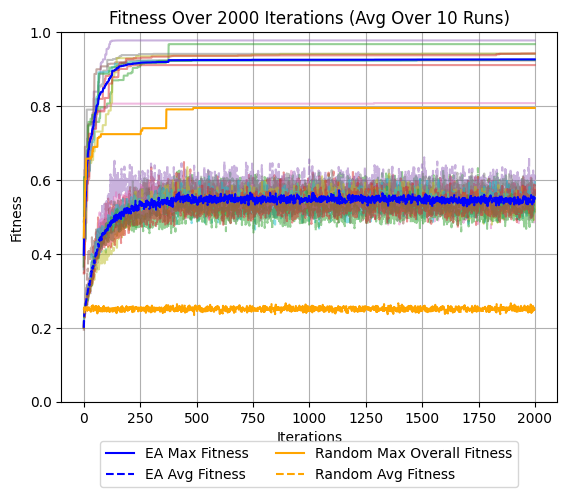
\includegraphics[width=.9\linewidth]{Project Report/Images/Simple Optimiser/2 Qubit/2 Qubit Simulation Fitness Chart.png}
  \caption{2 Qubit Circuits}
  \label{fig:sub1}
\end{subfigure}%
\begin{subfigure}{.5\textwidth}
  \centering
  \includegraphics[width=.9\linewidth]{Project Report/Images/Simple Optimiser/3 Qubit/3 Qubit Fitness Chart.png}
  \caption{3 Qubit Circuits}
  \label{fig:sub2}
\end{subfigure}
\caption{Convergence curves showing the average (dashed line) and maximum (solid line) fitness over iterations. Error bars represent the standard deviation across 20 runs.}
\label{fig:fitness_charts}
\end{figure}

In addition, box plots summarising the distribution of final fitness values are provided in Figure~\ref{fig:boxplots}. These plots illustrate the variability and consistency of the results obtained across multiple runs.

\begin{figure}[H]
\centering
\begin{subfigure}{.5\textwidth}
  \centering
  \includegraphics[width=.9\linewidth]{Project Report/Images/Simple Optimiser/2 Qubit/2 Qubit Simulation_box_plot.png}
  \caption{2 Qubit Circuits}
  \label{fig:sub1}
\end{subfigure}%
\begin{subfigure}{.5\textwidth}
  \centering
  \includegraphics[width=.9\linewidth]{Project Report/Images/Simple Optimiser/3 Qubit/3 Qubit Simulation_box_plot.png}
  \caption{3 Qubit Circuits}
  \label{fig:sub2}
\end{subfigure}
\caption{Box plots showing the final fitness distributions for 2-qubit and 3-qubit circuits.}
\label{fig:boxplots}
\end{figure}

\subsection{Results for Different Optimisation Approaches}
We evaluated three distinct fitness evaluation approaches: (i) noisy simulation, (ii) circuit depth reduction, and (iii) the combined approach. For each method, experiments were conducted for both 2- and 3-qubit circuits. Below, we briefly describe the results for each approach.

\subsubsection*{Noisy Simulation Approach:}
In this configuration, fitness was evaluated using state fidelity under a hardware-specific noise model. Figure~\ref{fig:noisy_fitness} displays the fitness distributions for this approach.

\begin{figure}[H]
\centering
\begin{subfigure}{.5\textwidth}
  \centering
  \includegraphics[width=.9\linewidth]{Project Report/Images/Noisy Optimiser/2 Qubit/2 Qubit Simulation Box Plot.png}
  \caption{2 Qubit Circuits}
  \label{fig:sub1}
\end{subfigure}%
\begin{subfigure}{.5\textwidth}
  \centering
  \includegraphics[width=.9\linewidth]{Placeholder}
  \caption{3 Qubit Circuits}
  \label{fig:sub2}
\end{subfigure}
\caption{Box plots for fitness values obtained using the noisy simulation approach for 2-qubit and 3-qubit circuits.}
\label{fig:noisy_fitness}
\end{figure}

\subsubsection*{Depth-Reduced Approach:}
For the depth-reduced approach, a penalty proportional to circuit depth was incorporated into the fitness function. The resulting fitness values, along with their variability, are summarised in Figure~\ref{fig:depth_fitness}.

\begin{figure}[H]
\centering
\begin{subfigure}{.5\textwidth}
  \centering
  \includegraphics[width=.9\linewidth]{Project Report/Images/Depth Optimiser/2 Qubit/2 Qubit Simulation_box_plot.png}
  \caption{2 Qubit Circuits}
  \label{fig:sub1}
\end{subfigure}%
\begin{subfigure}{.5\textwidth}
  \centering
  \includegraphics[width=.9\linewidth]{Placeholder}
  \caption{3 Qubit Circuits}
  \label{fig:sub2}
\end{subfigure}
\caption{Box plots for fitness values obtained using the depth-reduced approach for 2-qubit and 3-qubit circuits.}
\label{fig:depth_fitness}
\end{figure}

\subsubsection*{Combined Approach:}
The combined approach integrates both noise simulation and depth penalties. The fitness results for this configuration are shown in Figure~\ref{fig:combined_fitness}.

\begin{figure}[H]
    \centering
    \includegraphics[width=0.8\textwidth]{Project Report/Images/Placeholder_Image.png}
    \caption{Box plots for fitness values obtained using the combined approach for (a) 2-qubit and (b) 3-qubit circuits.}
    \label{fig:combined_fitness}
\end{figure}

\subsection{Comparative Analysis Under Various Conditions}
To assess the generalisability and robustness of the evolved circuits, we compared the top 10 circuits generated by each approach across all run of each simulation type. Table~\ref{tab:comparison} summarises the fitness values of the best circuits under:
\begin{itemize}
    \item Noiseless conditions.
    \item The specific noise simulator used for training.
    \item Unseen noise simulators.
\end{itemize}

\begin{table}[H]
    \centering
    \caption{Fitness comparison of the top 10 circuits (averaged over 20 runs) for 2- and 3-qubit circuits under various conditions.}
    \label{tab:comparison}
    \begin{tabular}{lcccc}
        \hline
        \textbf{Approach} & \textbf{Condition} & \textbf{Best Fitness} & \textbf{Mean Fitness} & \textbf{Std. Dev.} \\
        \hline
        Noisy Simulation & No Noise & [Placeholder] & [Placeholder] & [Placeholder] \\
        Noisy Simulation & Trained Noise & [Placeholder] & [Placeholder] & [Placeholder] \\
        Noisy Simulation & Unseen Noise & [Placeholder] & [Placeholder] & [Placeholder] \\
        \hline
        Depth-Reduced & No Noise & [Placeholder] & [Placeholder] & [Placeholder] \\
        Depth-Reduced & Trained Noise & [Placeholder] & [Placeholder] & [Placeholder] \\
        Depth-Reduced & Unseen Noise & [Placeholder] & [Placeholder] & [Placeholder] \\
        \hline
        Combined & No Noise & [Placeholder] & [Placeholder] & [Placeholder] \\
        Combined & Trained Noise & [Placeholder] & [Placeholder] & [Placeholder] \\
        Combined & Unseen Noise & [Placeholder] & [Placeholder] & [Placeholder] \\
        \hline
    \end{tabular}
\end{table}

\subsection{Structural Comparison of Evolved Circuits}
Beyond fitness metrics, we also analysed the structural differences between evolved circuits and the traditional QFT circuit. Figure~\ref{fig:structural_comp} illustrates representative circuit diagrams highlighting key differences in gate selection, parallelism, and circuit depth.

\begin{figure}[H]
    \centering
    \includegraphics[width=0.8\textwidth]{Project Report/Images/Placeholder_Image.png}
    \caption{Representative circuit diagrams comparing evolved circuits to the traditional QFT design.}
    \label{fig:structural_comp}
\end{figure}

\subsection{Discussion of Trade-offs and Statistical Analysis}
Our results demonstrate distinct trade-offs between the different approaches. The noisy simulation approach tends to excel under targeted noise conditions, while the depth-reduced approach shows higher generalisability under varied noise models. The combined approach attempts to balance these factors.

\subsubsection*{Statistical Analysis:}  
A preliminary statistical analysis (e.g., t-tests or ANOVA) indicates significant differences (p $<$ 0.05) in fitness outcomes between the approaches. Detailed statistical results and discussion will be presented in the Discussion section.

%%%%%%%%%%%%%%%%%%%%%%%%%%%%%%%%%%%%%%%%%%%%%%%%%%%%%%%%%%%%%%%%%%%%%%
%
%    Discussion & Critical Analysis
%
%%%%%%%%%%%%%%%%%%%%%%%%%%%%%%%%%%%%%%%%%%%%%%%%%%%%%%%%%%%%%%%%%%%%%%
\section{Discussion \& Critical Analysis}

(Approximately 3 pages) Reflect on your project outcomes.

\begin{itemize}
    \item Summarise the key findings and how each experimental variant performed.
    \item Discuss the impact of incorporating noise simulation and circuit depth into the fitness evaluation.
    \item Reflect on the strengths and weaknesses of your approach, including challenges in EA convergence and simulation limitations.
    \item Consider the feedback received on your literature review and project plan, and discuss how your approach addresses or could further refine the objectives.
\end{itemize}

%%%%%%%%%%%%%%%%%%%%%%%%%%%%%%%%%%%%%%%%%%%%%%%%%%%%%%%%%%%%%%%%%%%%%%
%
%    Conclusions & Future Work
%
%%%%%%%%%%%%%%%%%%%%%%%%%%%%%%%%%%%%%%%%%%%%%%%%%%%%%%%%%%%%%%%%%%%%%%
\section{Conclusions \& Future Work}

(Approximately 2 pages) Conclude your report with a summary and future directions.

\begin{itemize}
    \item Recap the main contributions and findings of your project.
    \item State which experimental configuration yielded the best trade-off between fidelity and noise resilience.
    \item Propose avenues for future work, such as testing on real quantum hardware or applying the approach to other quantum algorithms.
\end{itemize}

%%%%%%%%%%%%%%%%%%%%%%%%%%%%%%%%%%%%%%%%%%%%%%%%%%%%%%%%%%%%%%%%%%%%%%
%
%    References
%
%%%%%%%%%%%%%%%%%%%%%%%%%%%%%%%%%%%%%%%%%%%%%%%%%%%%%%%%%%%%%%%%%%%%%%
\addcontentsline{toc}{section}{References} % Add References to the table of contents
\printbibliography

%%%%%%%%%%%%%%%%%%%%%%%%%%%%%%%%%%%%%%%%%%%%%%%%%%%%%%%%%%%%%%%%%%%%%%
%
%    Appendices (Optional)
%
%%%%%%%%%%%%%%%%%%%%%%%%%%%%%%%%%%%%%%%%%%%%%%%%%%%%%%%%%%%%%%%%%%%%%%
\newpage
\appendix
\section*{Appendix A}
\addcontentsline{toc}{section}{Appendix A} % Add Appendix A to the table of contents

PLACEHOLDER FOR ADDITIONAL MATERIAL, SUCH AS SIMULATION LOGS, CODE SNIPPETS, OR DETAILED EXPERIMENTAL SETTINGS.

\end{document}
